\documentclass[../main.tex]{subfiles}
\chapter{Herleitung}
\label{c:herleitung}

\section[Operatoren]{Operatoren für Transformationen}
\subsection{Translation}
\begin{equation}
	T_{\mathbf{v}} \begin{pmatrix}t_x\\t_y\\t_z\\\end{pmatrix}= \begin{bmatrix}1 & 0 & 0 & t_x\\0 & 1 & 0 & t_y\\0 & 0 & 0 & t_z\\0 & 0 & 0 & 1\end{bmatrix}
\end{equation}

\subsection{Rotation}
\begin{equation}
	\begin{split}
		R = & R_{z}(\alpha )\,R_{y}(\beta )\,R_{x}(\gamma ) \\
		= & \begin{bmatrix}\cos \alpha & -\sin \alpha & 0\\\sin \alpha & \cos \alpha & 0\\0& 0& 1\\\end{bmatrix}
			\begin{bmatrix}\cos \beta & 0& \sin \beta \\0& 1& 0\\-\sin \beta & 0& \cos \beta \\\end{bmatrix}
			\begin{bmatrix}1& 0& 0\\0& \cos \gamma & -\sin \gamma \\0& \sin \gamma & \cos \gamma \\\end{bmatrix} \\
		= & \begin{bmatrix}
			\cos \alpha \cos \beta & \cos \alpha \sin \beta \sin \gamma -\sin \alpha \cos \gamma & \cos 	\alpha \sin \beta \cos \gamma +\sin \alpha \sin \gamma \\
			\sin \alpha \cos \beta & \sin \alpha \sin \beta \sin \gamma +\cos \alpha \cos \gamma & \sin \alpha \sin \beta \cos \gamma -\cos \alpha \sin \gamma \\
			-\sin \beta & \cos \beta \sin \gamma & \cos \beta \cos \gamma \\
		\end{bmatrix}
	\end{split}
\end{equation}

\subsection[Transformationsmatrix]{Homogene Transformationsmatrix}
Die Anordnung eines körperfesten Koordinatensystems $\{b\}$ (body-frame) in einem raumfesten Koordinatensystem $\{s\}$ (space-frame) kann beschrieben werden durch die Position des body-frames $p$ in $\{s\}$-Koordinaten und einer Rotationsmatrix $R$, welche die Ausrichtung von $\{b\}$ in $\{s\}$-Koordinaten.
\begin{equation}
	T = \begin{bmatrix}R & p\\0 & 1\end{bmatrix} = \begin{bmatrix}r_{11} & r_{12} & r_{13} & p_1\\r_{21} & r_{22} & r_{23} & p_2\\r_{31} & r_{32} & r_{33} & p_3\\0 & 0 & 0 & 1\end{bmatrix}
\end{equation}

\section[Maschine]{Kinematik der Maschine}

\begin{figure}
	\centering
	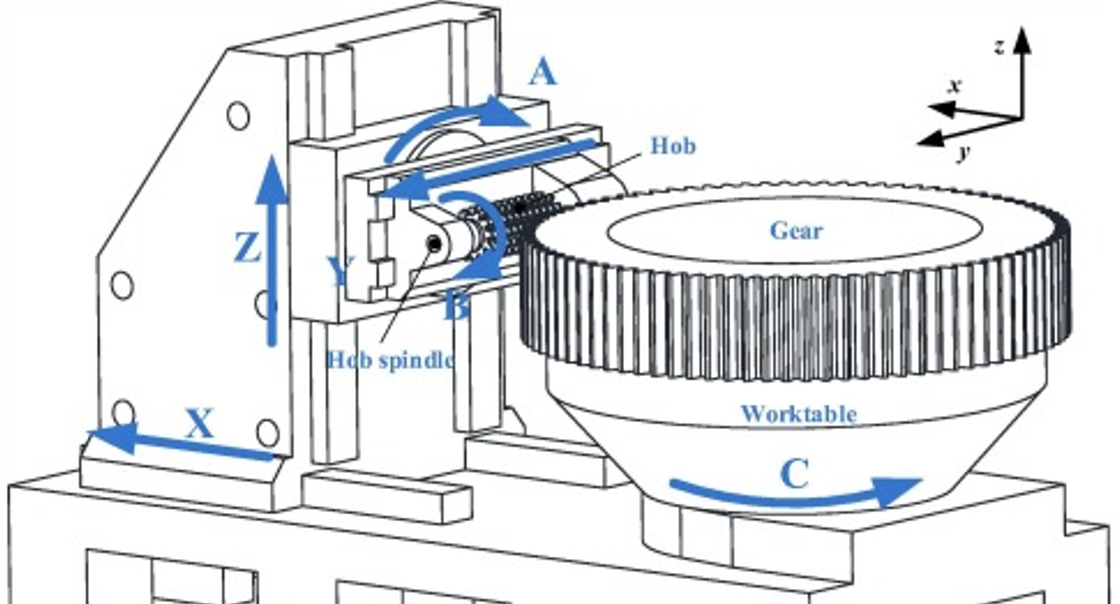
\includegraphics[width=12cm]{maschine_frei}
	\label{fig:maschine}
	\caption{Kinematik der Maschine mit Vorzeichenrichtung der Achsen}
\end{figure}


\begin{equation}
	\mathbf{p}_m = T_{\mathbf{v}} \begin{pmatrix}a\\b\\c\\\end{pmatrix} \cdot{} R \begin{pmatrix}0\\0\\C - \gamma\\\end{pmatrix} \cdot{} \mathbf{p}_{WSt}
\end{equation}